\begin{tikzpicture}
\draw[-latex] (0,0) -- (15,0);
\draw[-latex] (0,0) -- (0,15);
\foreach \x in {1,2,...,14} {
  \draw (\x,0.1) -- (\x,-0.1);
  \draw (-0.1,\x) -- (0.1,\x);
}
%\draw (2,3) -- (10,6) -- (11,11) -- (3,10) -- (2,3);
\node at (12,3) {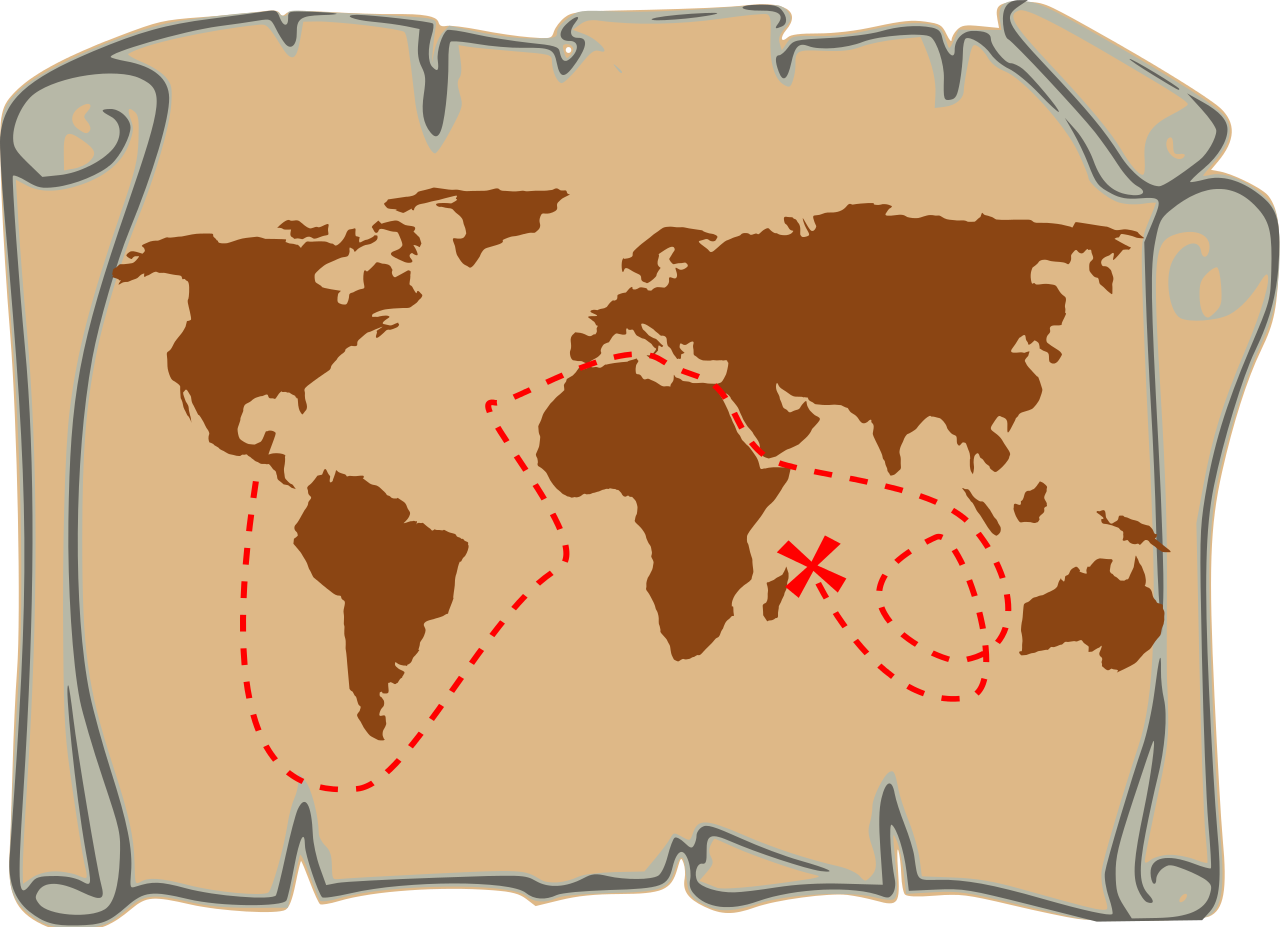
\includegraphics[width=1in]{assets/clipart/map.png}};
\node at (4,6) {
\includegraphics[width=1in]{assets/clipart/hat.png}};
\node at (8,8) {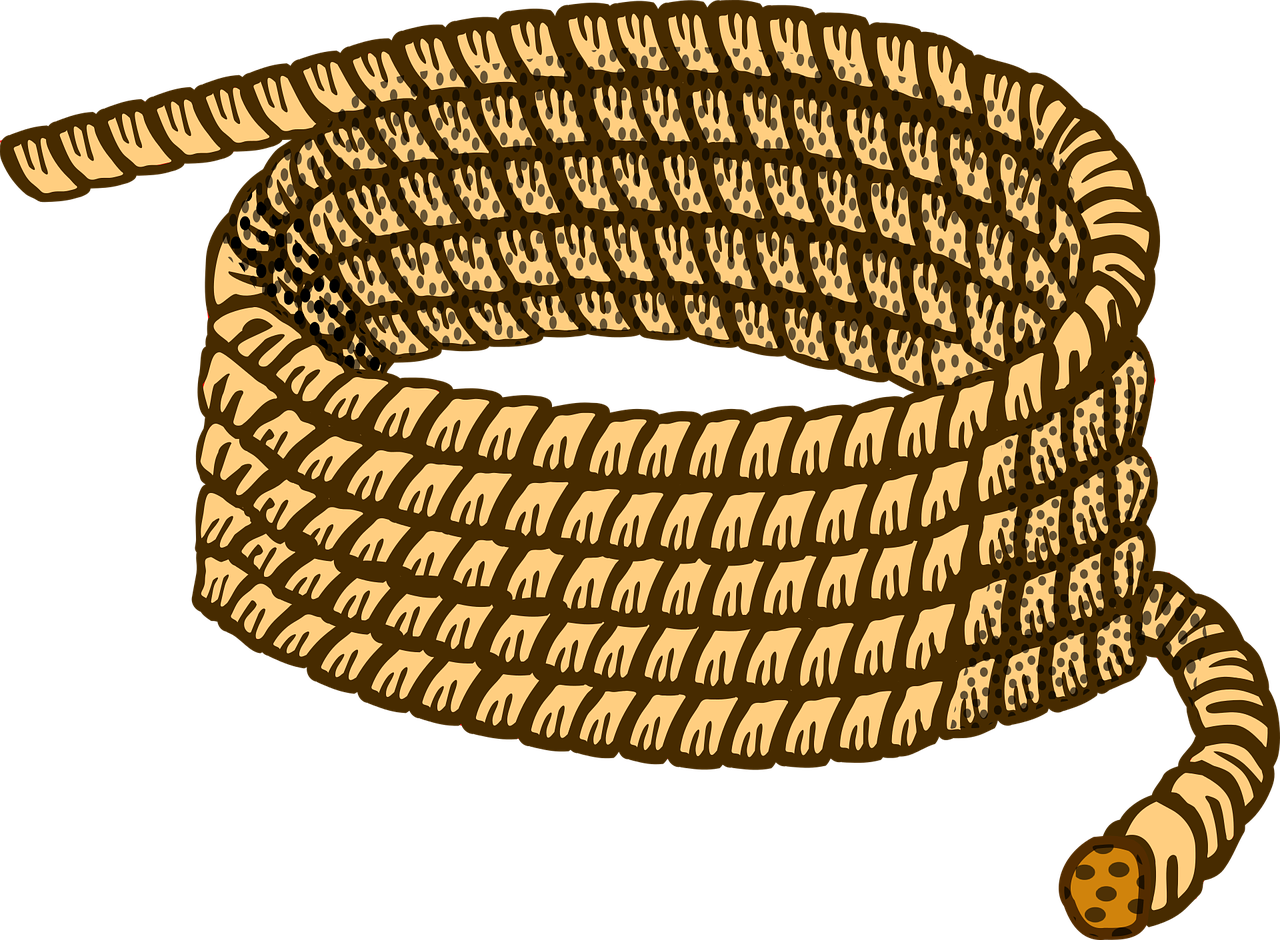
\includegraphics[width=1in]{assets/clipart/rope.png}};
\node at (3,12) {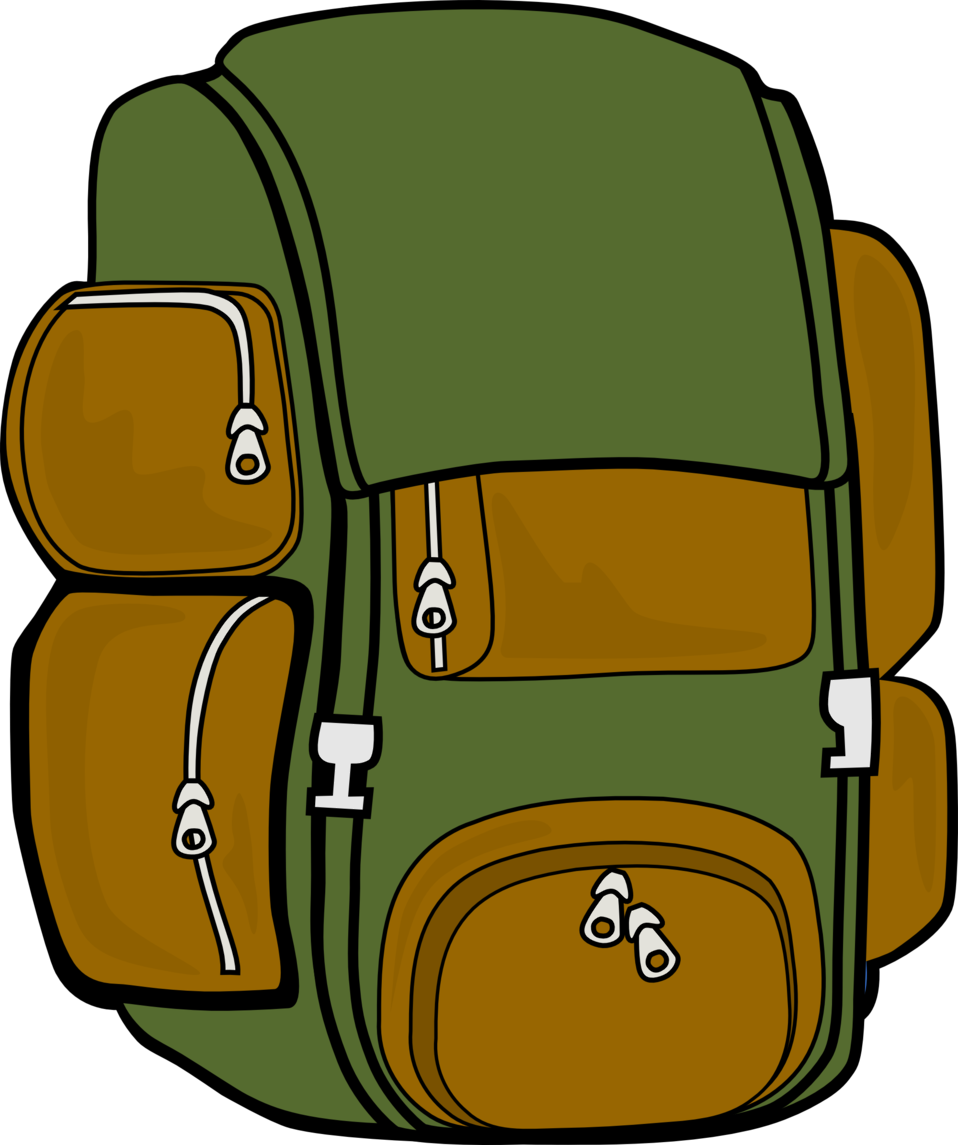
\includegraphics[width=1in]{assets/clipart/backpack.png}};
\node at (13,7) {
\includegraphics[width=1in]{assets/clipart/compass.png}};
\node at (7,2) {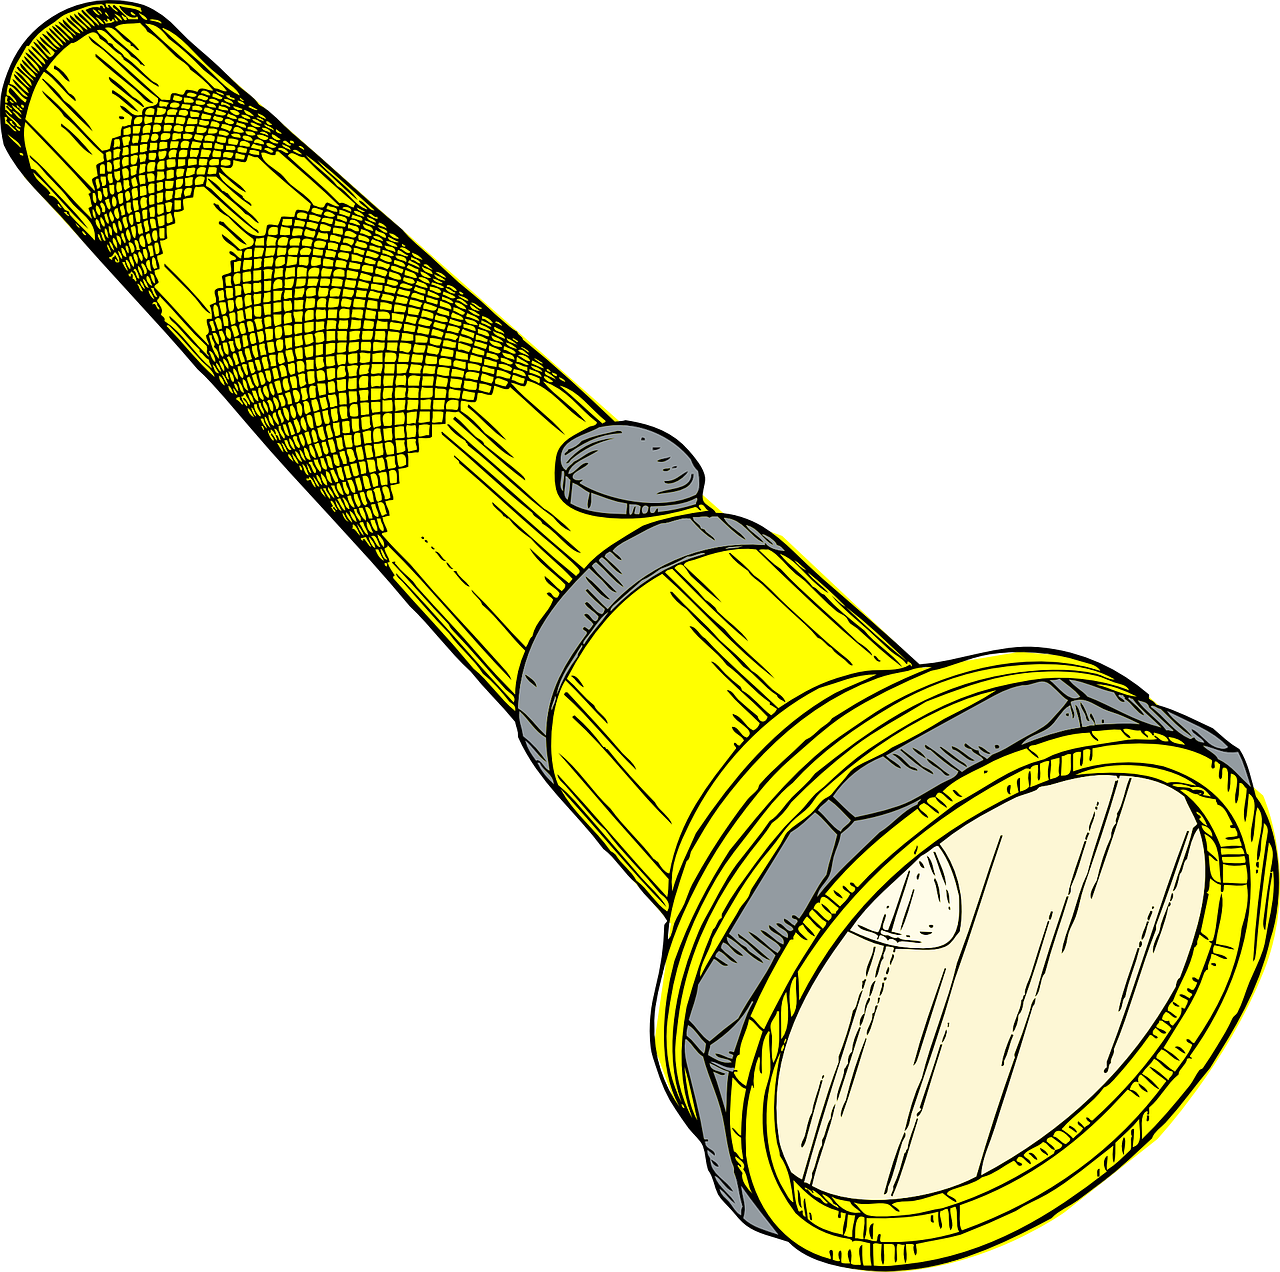
\includegraphics[width=1in]{assets/clipart/flashlight.png}};
\end{tikzpicture}

\vfill
{\LARGE\normalfont\wedn
Site Adjustment:
\begin{enumerate}
\item Site 1: \((?,?) + (-4,-16)\)
\item Site 2: \((?,?) + (6,-15)\)
\item Site 3: \((?,?) + (5,-1)\)
\item Site 4: \((?,?) + (-3,-1)\)
\end{enumerate}
}

\vfill
